\section{Herramientas de operación}\label{sec:herramientas}

Un clúster en marcha necesita dos cosas más que resolver páginas: observar su estado sin alterarlo y ejercitar los mecanismos que no aparecen en una carga normal. \texttt{dsmctl} cubre la observación, los reportes HTML convierten esa observación en un documento legible y \texttt{demo} reúne las demostraciones de coherencia, ejecución distribuida y paridad. Las tres herramientas usan la API y los mensajes públicos; ninguna necesita un modo especial del nodo ni acceso al interior de sus estructuras.

\subsection{\texttt{dsmctl}}\label{sec:dsmctl}

\texttt{dsmctl} es un cliente de diagnóstico que no integra la membresía. Abre una conexión TCP efímera al puerto de escucha de un nodo, envía una petición \texttt{QUERY\_REQ} y lee la respuesta \texttt{QUERY\_RESP}; el listener del nodo atiende una sola trama por conexión y la cierra al responder, así que cada consulta usa su propio socket. El nodo no registra al consultor como miembro ni le reserva marcos de memoria, de modo que consultar no cambia la membresía, el tamaño del clúster ni las páginas de nadie. La configuración aporta el \texttt{cluster\_id} que valida la respuesta y el puerto por defecto; sin \texttt{-{}-port}, la herramienta consulta \texttt{PORT\_MIN}, que es el puerto que toma el primer nodo de la máquina si está libre. Las opciones \texttt{-c} o \texttt{-{}-conf}, \texttt{-H} o \texttt{-{}-host} y \texttt{-p} o \texttt{-{}-port} se aceptan antes o después del comando; el host por omisión es \texttt{127.0.0.1}.

\begin{lstlisting}[language=bash, caption={Consultas de \texttt{dsmctl} sobre un clúster en marcha.}, label={lst:dsmctl}]
./build/bin/release/dsmctl --conf dsm.conf nodes
./build/bin/release/dsmctl --conf dsm.conf stats
./build/bin/release/dsmctl --conf dsm.conf pages 0 16
./build/bin/release/dsmctl --conf dsm.conf dir 0 16
./build/bin/release/dsmctl --conf dsm.conf alloc
./build/bin/release/dsmctl --conf dsm.conf html /tmp/informes
./build/bin/release/dsmctl --conf dsm.conf config
\end{lstlisting}

\texttt{nodes} muestra la tabla de membresía del nodo contactado. Cada fila lleva la ranura, el UUID, la dirección IP, el puerto TCP, el rol, el estado, las páginas aportadas, las páginas libres del clúster, los latidos perdidos y la época. La ranura es el identificador de la membresía vigente que usan los mensajes y el anillo; el UUID distingue la identidad aunque la ranura cambie; el rol separa a un nodo que aporta memoria de un cliente que solo usa la vista. Las páginas aportadas se expresan en páginas de 4 KiB, no en bytes: 16\,384 páginas equivalen a 64 MiB. Los latidos perdidos cuentan transiciones a \texttt{SUSPECT} y \texttt{DEAD}, no cada intervalo en que un nodo llega tarde. Al final, la herramienta separa \texttt{Nodos listados} de \texttt{Clientes listados}, de modo que un cliente no infla el total de nodos. La tabla refleja la membresía que conoce el nodo consultado; un nodo declarado muerto desaparece de esa vista.

\texttt{stats} recorre la tabla de membresía, consulta las estadísticas de cada miembro que responde y presenta una fila por miembro con ranura, rol, fallos de lectura, fallos de escritura, mensajes, deltas de paridad, franjas reconstruidas y latidos perdidos. Después suma los contadores y muestra los totales agregados: fallos de lectura y escritura, fallos totales, mensajes enviados y recibidos, bytes enviados y recibidos con su equivalencia en KiB o MiB, tareas distribuidas correctas y fallidas, deltas de paridad, franjas reconstruidas, respuestas descartadas y latidos perdidos. La columna \texttt{Mensajes} de la tabla por nodo es la suma de enviados y recibidos; el agregado los separa. Si un miembro no responde, la herramienta lo informa y continúa con los demás, y la línea \texttt{Nodos consultados} indica cuántos de los listados aportaron datos. Los clientes también responden a la consulta y sus contadores entran en el agregado, aunque no aporten memoria.

\texttt{pages} tiene dos partes. Sin argumentos, recorre la tabla local del nodo contactado y resume el total de páginas de la vista, las que están en \texttt{M}, las que están en \texttt{S}, las que están en \texttt{I} y las transiciones pendientes \texttt{IS\_PEND}, \texttt{IM\_PEND} y \texttt{SM\_PEND}. El total es el tamaño de la vista dividido entre el tamaño de página, 1\,048\,576 páginas con los valores por omisión, no la cantidad de páginas con datos; la mayor parte suele estar en \texttt{I}. Con un rango, \texttt{pages inicio n} imprime el directorio global de ese intervalo. \texttt{dir inicio n} muestra el mismo directorio sin el resumen. En ambos, las columnas son página, propietario, proceso, orden, copyset y franja; el propietario es el custodio que calcula el anillo, el proceso es el PID que reservó el bloque, el orden es el índice de la página dentro de esa reserva, el copyset es el conjunto de ranuras con copia válida en \texttt{S} o \texttt{M} y la franja agrupa las páginas en el reporte y, con redundancia, en la paridad. Cuando se pide un rango sin indicar cantidad, \texttt{pages} y \texttt{dir} usan 16 páginas, porque la vista completa supera el millón de páginas y enumerarla sin acotar produce una salida inmanejable.

\texttt{alloc} lista los bloques reservados del espacio global. Cada fila contiene la primera página, la cantidad de páginas, el proceso que hizo la reserva (o \texttt{-} si no tiene PID), la ranura y el identificador de la reserva. La herramienta filtra las entradas que ya no están vivas, de modo que la tabla muestra el estado vigente y no el historial. El rango por omisión es de 32 bloques. Esta consulta sirve para relacionar una página del directorio con la aplicación que la reservó: el PID y el orden que aparecen en \texttt{dir} provienen de la misma reserva que \texttt{alloc} enumera.

\texttt{html} pide al nodo consultado que genere el informe en un directorio. Sin argumento usa \texttt{OUTPUT\_DIR} de la configuración; con un argumento usa esa ruta. El nodo crea el directorio si no existe, escribe \texttt{global.html} y un archivo \texttt{nodo-<ranura>.html} por cada nodo que aporta memoria, y responde con la ruta y el patrón de nombres. La generación ocurre en el sistema de archivos del nodo consultado, no en el de la máquina desde la que se ejecuta \texttt{dsmctl}; si el nodo corre en otra computadora, los archivos quedan allí.

\texttt{config} no consulta al clúster: lee el archivo de configuración con el que se invoca la herramienta y muestra el identificador de clúster, el tamaño de página, la dirección base, el tamaño de vista, la memoria por nodo, los nodos máximos, los nodos virtuales por MiB, la redundancia, el rango de puertos, el grupo y puerto de descubrimiento, los plazos de conexión, descubrimiento, envío y solicitud, los reintentos, los parámetros de latido, los hilos trabajadores y despachadores, las franjas de cerrojo, el margen de custodio, el plazo de cerrojo, la capacidad de la cola, el nivel de registro y el hash de configuración compartida. Si se indica un puerto fuera del rango declarado, agrega un aviso.

\subsection{Reportes HTML globales y por nodo}\label{sec:reportes-html}

El informe HTML se arma con la misma información que consulta \texttt{dsmctl}, pero en el nodo que lo genera. \texttt{dsm\_html\_report} reúne la membresía viva, consulta la tabla de páginas de cada miembro y escribe dos tipos de archivo. \texttt{global.html} contiene los metadatos del clúster, la lista de nodos y clientes y una tabla global de páginas materializadas. Cada \texttt{nodo-<ranura>.html} contiene los datos de ese nodo, sus estadísticas locales si es el nodo que genera el informe y su tabla de páginas con el estado MSI. Un cliente aparece en la lista global con rol \texttt{cliente}, cero páginas y sin enlace a un archivo propio, porque no aporta memoria ni custodia páginas. Los archivos por nodo se generan solo para los miembros que aportan memoria.

\begin{figure}[H]
\centering
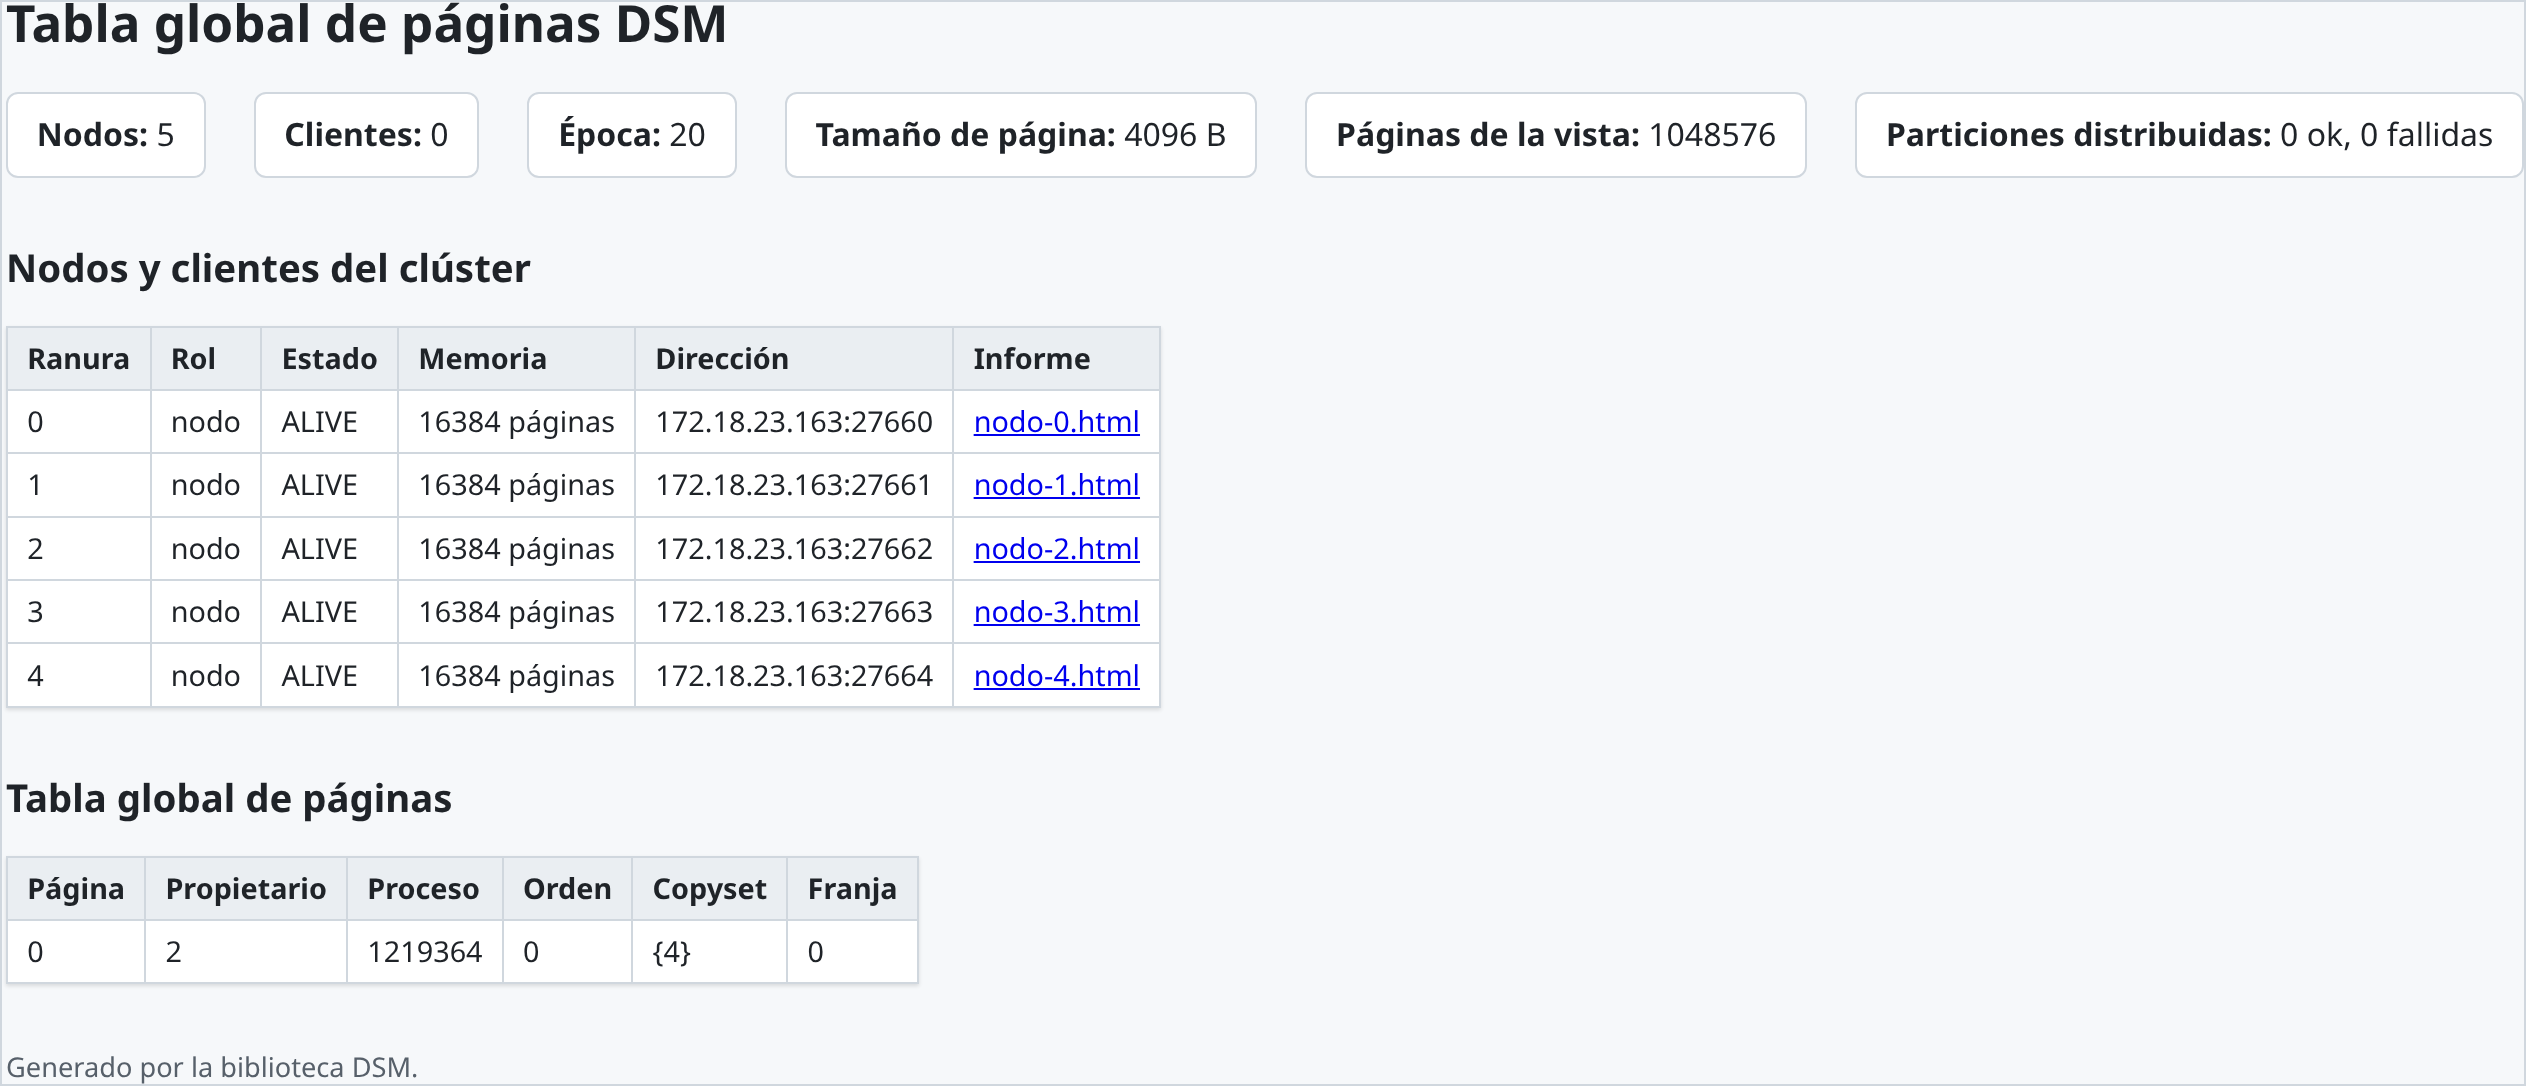
\includegraphics[width=\linewidth]{figuras/html-global.png}
\caption{Reporte global de páginas del clúster.}
\label{fig:html-global}
\end{figure}

La figura~\ref{fig:html-global} muestra un reporte global de una corrida local. Los recuadros superiores resumen cinco nodos, cero clientes, época 20, tamaño de página de 4096 B, 1\,048\,576 páginas de vista y cero particiones distribuidas correctas o fallidas. La lista de miembros tiene cinco filas, todas con rol \texttt{nodo}, estado \texttt{ALIVE}, 16\,384 páginas aportadas (64 MiB) y direcciones de la misma máquina en los puertos 27660 a 27664; cada fila enlaza su archivo \texttt{nodo-<ranura>.html}. La tabla global contiene una página materializada: la página 0, con propietario 2, proceso 1219364, orden 0, copyset \texttt{\{4\}} y franja 0.

Esa fila permite leer la diferencia entre custodio y copia. El propietario es la ranura que el anillo de dispersión asigna como home de la página; el copyset es el conjunto de ranuras que en ese momento tienen una copia válida en \texttt{S} o \texttt{M}. En la captura, el home es la ranura 2 y la única copia está en la ranura 4, de modo que el directorio de la página vive en 2 mientras el contenido modificado vive en 4. El proceso 1219364 es el PID que reservó el bloque, no el nodo que lo custodia; el orden 0 indica que la página es la primera de esa reserva, y la franja 0 que pertenece al primer grupo que usa el reporte. La tabla global no muestra el estado MSI porque cada nodo tiene el suyo para la misma página; esa información aparece en el archivo del nodo que conserva la copia.

\begin{figure}[H]
\centering
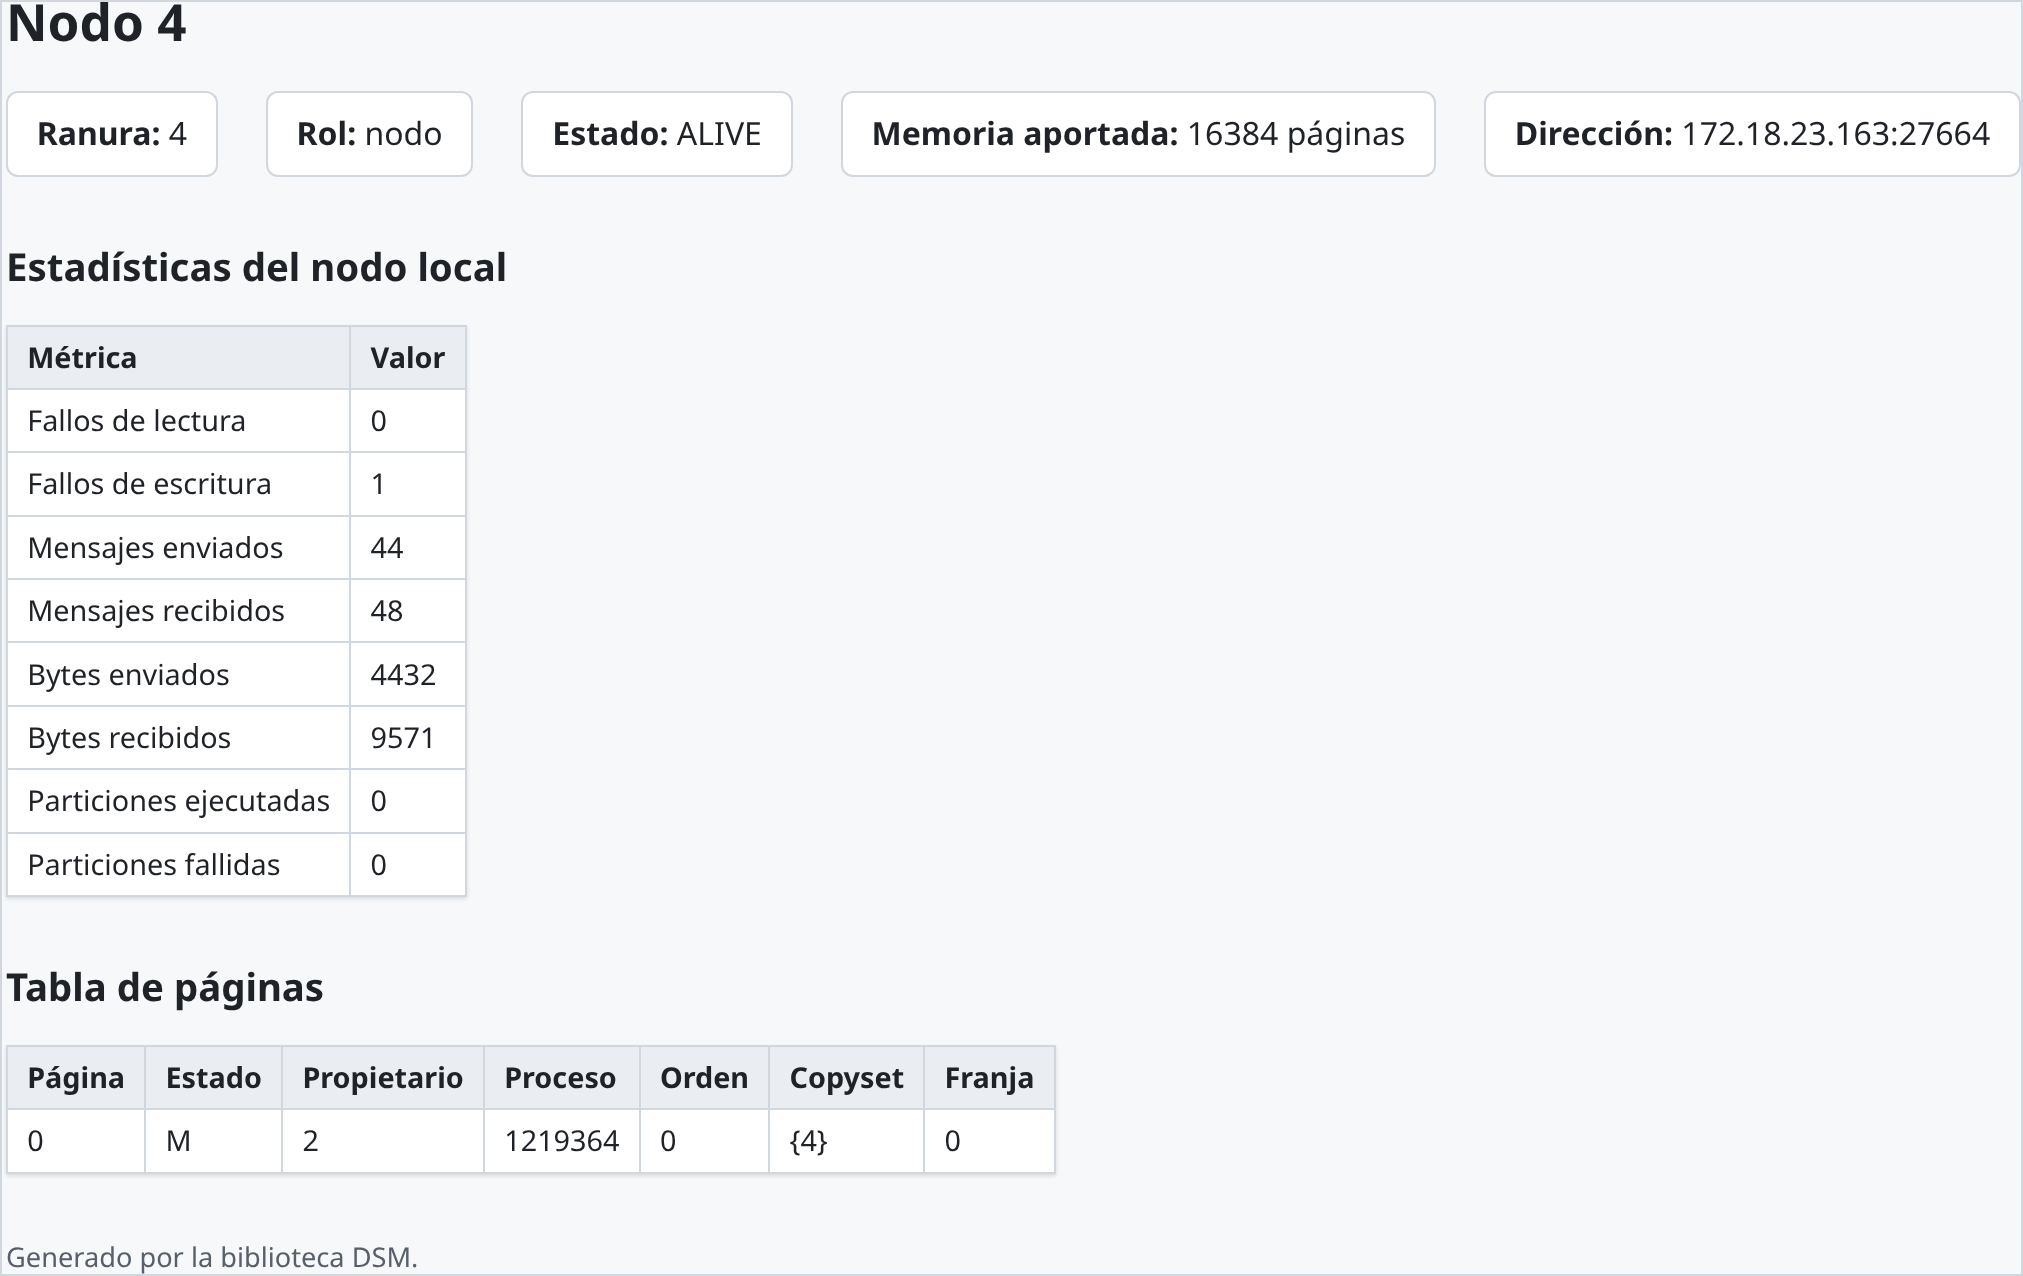
\includegraphics[width=\linewidth]{figuras/html-nodo.png}
\caption{Reporte de un nodo con una página en estado M.}
\label{fig:html-nodo}
\end{figure}

La figura~\ref{fig:html-nodo} corresponde al archivo del nodo 4 de la misma corrida. Los recuadros repiten ranura 4, rol \texttt{nodo}, estado \texttt{ALIVE}, 16\,384 páginas aportadas y la dirección 172.18.23.163:27664. Las estadísticas del nodo local registran 0 fallos de lectura, 1 fallo de escritura, 44 mensajes enviados, 48 recibidos, 4432 bytes enviados, 9571 bytes recibidos y 0 particiones ejecutadas o fallidas. La tabla de páginas tiene una fila: página 0, estado \texttt{M}, propietario 2, proceso 1219364, orden 0, copyset \texttt{\{4\}} y franja 0. El estado \texttt{M} confirma que la copia de la ranura 4 es la única válida y que está modificada; el propietario 2 sigue siendo el custodio del directorio.

Los nombres de las columnas se leen así. \textbf{Ranura} es la posición del miembro en la membresía, un número entre 0 y \texttt{MAX\_NODES}-1 que identifica al nodo en los mensajes y en el anillo. \textbf{Rol} distingue \texttt{nodo} de \texttt{cliente}: el primero aporta páginas y puede ser custodio, el segundo usa la vista sin aportar memoria. \textbf{Estado} en la lista de miembros vale \texttt{ALIVE}, \texttt{SUSPECT} o \texttt{DEAD}; en la tabla de páginas vale \texttt{M}, \texttt{S}, \texttt{I} o uno de los transitorios \texttt{IS\_PEND}, \texttt{IM\_PEND} y \texttt{SM\_PEND}. \textbf{Memoria} es la cantidad de páginas aportadas, que multiplicada por 4096 B da los MiB del nodo. \textbf{Dirección} es la IP y el puerto TCP de escucha. \textbf{Página} es el índice de la página dentro de la vista, no una dirección virtual: la dirección correspondiente es la base de la vista más \texttt{página} $\times$ 4096. \textbf{Propietario} es la ranura del custodio que asigna el anillo, no necesariamente la que tiene la copia. \textbf{Proceso} es el PID que reservó el bloque, o \texttt{-} si la página todavía no pertenece a ninguna reserva. \textbf{Orden} es el índice de la página dentro de esa reserva. \textbf{Copyset} es el conjunto de ranuras con copia válida en \texttt{S} o \texttt{M}; una página sin copia se muestra como \texttt{-}. \textbf{Franja} es el grupo que usa el reporte y, con redundancia activa, la paridad: en ese modo se calcula como página dividida entre $K$, con $K$ igual a los nodos vivos menos uno y acotado entre 2 y 8; sin redundancia se calcula como página dividida entre \texttt{CHUNK\_PAGES}, que vale 4 por omisión.

El reporte global y el de un nodo no son dos copias del mismo documento. El global omite el estado MSI y solo imprime las páginas que tienen al menos una copia, porque su objetivo es mostrar qué hay materializado en el clúster y quién lo tiene. El archivo por nodo imprime las páginas que ese nodo ve con estado distinto de \texttt{I}, incluye la columna \texttt{Estado} y añade las estadísticas locales cuando el archivo corresponde al nodo que genera el informe. Los clientes no tienen archivo propio, pero su tabla local se consulta para recuperar el PID y el orden reales de las páginas que conservan; por eso un copyset puede incluir una ranura de cliente aunque esa ranura no aparezca como nodo ni tenga archivo.

La generación tiene dos topes operativos. Recorre solo rangos de páginas materializadas, hasta 1024 rangos y 4096 filas, para que una vista de un millón de páginas con pocos datos no convierta el informe en una consulta sin fin. Las páginas en \texttt{I} no se escriben en el archivo por nodo, y las que no tienen copia no se escriben en el global. El recuadro \texttt{Páginas de la vista} indica el tamaño de la vista en páginas, no la cantidad de filas del informe; una vista de 1\,048\,576 páginas puede producir una tabla de una sola fila. El recuadro \texttt{Particiones distribuidas} cuenta las particiones que ejecutó el nodo que genera el informe, no la suma del clúster, porque se obtiene de \texttt{dsm\_stats} local.

\subsection{\texttt{demo}: coherencia, ejecución distribuida y paridad}\label{sec:demo}

\texttt{demo} reúne seis roles que se eligen con dos palabras en la línea de comandos. Los roles \texttt{dist coord} y \texttt{dist worker} ejercitan el registro de kernels y el reparto de particiones; \texttt{raid hold} y \texttt{raid produce} ejercitan la paridad y la reconstrucción; \texttt{msi a} y \texttt{msi b} ejercitan la coherencia entre dos procesos. Cada rol fija una etiqueta de nodo distinta para que varios procesos de la misma máquina no compartan identidad: \texttt{dist\_coord}, \texttt{dist\_worker}, \texttt{raid\_hold\_<pid>}, \texttt{raid\_producer\_<pid>}, \texttt{msi\_a\_<pid>} y \texttt{msi\_b\_<pid>}. Los roles que permanecen a la espera leen órdenes por la entrada estándar: \texttt{dist coord} acepta \texttt{LAUNCH <ranura>}, \texttt{raid hold} acepta \texttt{READ} y \texttt{READPAGE}, y \texttt{msi a} y \texttt{msi b} aceptan \texttt{READ} y \texttt{QUIT}; \texttt{dist worker} espera trabajo y \texttt{raid produce} recibe las páginas y los nodos como argumentos. Las respuestas empiezan por un marcador, y ese formato es el que usan las pruebas de extremo a extremo para controlar los procesos sin intervención manual.

\paragraph{\texttt{dist coord}.} Se une como nodo, reserva cuatro páginas (16 KiB), registra el kernel \texttt{0x44495354} y publica \texttt{COORD\_READY} con su ranura, la dirección virtual del bloque y el tamaño. Después lee líneas \texttt{LAUNCH <ranura>} y reparte ocho particiones de 1024 bytes entre su propia ranura y la ranura remota indicada. Los primeros 8 KiB del bloque contienen la fuente y los 8 KiB siguientes el destino; cada partición describe un rango de 1024 bytes en ambas regiones. El kernel aplica una XOR con la clave \texttt{0x5A}, de modo que el contenido de salida depende del código registrado en cada proceso y no de una simple copia. El coordinador lanza el trabajo, recoge los resultados, calcula el XOR de los CRC32 de las particiones de destino y llama a \texttt{dsm\_dist\_verify} y comprueba el patrón byte por byte. Al final imprime \texttt{DIST\_SLOTS}, una línea \texttt{DIST\_PART} por partición con ranura, origen, elementos y microsegundos, y \texttt{DIST PASS} o \texttt{DIST FAIL} con las claves \texttt{remote}, \texttt{total}, \texttt{verify} y \texttt{lectura}. La orden \texttt{QUIT} cierra el proceso.

\paragraph{\texttt{dist worker}.} Se une como nodo, registra el mismo kernel y publica \texttt{WORKER\_READY} con su ranura. No lanza trabajo: espera las órdenes \texttt{DIST\_RUN} que llegan por la red, ejecuta el kernel en el hilo trabajador que atendió el mensaje, calcula el CRC32 del rango de salida y responde \texttt{DIST\_DONE} con el estado, los elementos, el CRC, la duración y los fallos de lectura y escritura. El coordinador puede ejecutar sus propias particiones sin abrir una conexión contra su listener, así que el reparto por turno produce cuatro particiones locales y cuatro remotas cuando hay un trabajador. La orden \texttt{QUIT} lo cierra.

\paragraph{\texttt{raid hold}.} Se une como nodo y publica \texttt{HOLD\_READY} con su ranura. Después acepta \texttt{READPAGE 0x<va> <índice>} para comprobar una página o \texttt{READ 0x<va> <páginas>} para comprobar un rango completo. El patrón de cada página depende del índice y del desplazamiento: \texttt{(página} $\times$ 131 + \texttt{offset} $\times$ 17 + \texttt{0x5A) \& 0xFF}. Cada comprobación responde \texttt{PASS} o \texttt{FAIL}; la orden \texttt{QUIT} termina el proceso. Los procesos \texttt{hold} representan a los nodos que aportan memoria y permanecen vivos mientras el productor escribe y sincroniza.

\paragraph{\texttt{raid produce}.} Espera a que la membresía reúna la cantidad de nodos indicada, con un plazo de 30 s, reserva la cantidad de páginas pedida, escribe el mismo patrón página por página, llama a \texttt{dsm\_sync}, vuelve a leer el bloque y publica \texttt{RAID\_READY} con la dirección virtual, las páginas, su ranura, el resultado de la sincronización, el resultado de la lectura y los deltas de paridad locales. Si se ejecuta con \texttt{DSM\_NODE\_MODE=client}, no aporta memoria ni custodia páginas; las pruebas lo lanzan así para que los tres nodos \texttt{hold} sean los únicos custodios. El productor termina después de publicar la línea, de modo que ninguna copia local sobrevive; los \texttt{hold} pueden leer el bloque con la dirección publicada porque comparten la misma vista.

\paragraph{\texttt{msi a} y \texttt{msi b}.} El rol \texttt{a} reserva una página, la llena con el patrón \texttt{0xA0000000 + i} por cada palabra de 32 bits, publica \texttt{A\_READY PASS} con la dirección virtual y espera la orden \texttt{READ}. El rol \texttt{b} recibe esa dirección por argumento, se enlaza al DSM, lee la página y comprueba el patrón de A; después escribe el patrón \texttt{0xB0000000 + i} y publica \texttt{B\_AFTER\_WRITE PASS}. Cuando A recibe \texttt{READ}, vuelve a leer la página y comprueba el patrón de B. Si B obtuvo una copia modificada, A queda sin copia válida y su acceso produce un fallo de lectura que el despachador resuelve con el contenido nuevo. Los dos roles imprimen sus estadísticas antes y después de cada paso, y la orden \texttt{QUIT} los cierra.

La corrida de extremo a extremo confirma los tres mecanismos. La ejecución distribuida termina con \texttt{DIST PASS remote=4 total=8 verify=ok lectura=ok}, es decir, cuatro de las ocho particiones se ejecutaron en el trabajador remoto, las ocho se recogieron, el CRC agregado coincidió y la lectura del destino reprodujo el patrón. La prueba de paridad reconstruye 6 franjas y verifica 5 páginas después de la caída de un nodo. El flujo MSI entre dos procesos termina en \texttt{PASS}: B lee el patrón de A, lo modifica, A vuelve a fallar para leer el valor nuevo y las estadísticas muestran fallos de lectura y fallos atendidos. Estos resultados no se imprimen como un adorno: cada uno exige que el mecanismo haya hecho su trabajo, porque el patrón o el CRC fallarían si la página se hubiera servido mal.

\subsection{Interpretación de métricas y reportes}\label{sec:metricas}

Los contadores de \texttt{dsm\_stats} son acumulados del proceso desde \texttt{dsm\_init} hasta el momento de la consulta. \texttt{dsmctl stats} los suma recorriendo los miembros que responden, de modo que el agregado representa lo observado por esos procesos y no una verdad única del clúster. Un nodo que no contesta queda fuera de la suma, y un cliente que responde aporta sus contadores aunque no aporte memoria. El informe HTML, en cambio, usa las estadísticas del nodo que lo genera; por eso el recuadro de particiones distribuidas puede ser cero aunque otro nodo haya ejecutado trabajo.

Las fallas de lectura y escritura cuentan los accesos que dispararon \texttt{SIGSEGV} y que el despachador atendió. Una falla de lectura aparece cuando el proceso toca una página que no tiene o que fue invalidada; una de escritura aparece en la primera escritura sobre una página que estaba en \texttt{I} o en \texttt{S}. Al inicio de una aplicación las fallas crecen con las páginas que se materializan, y en régimen estable se estabilizan. Las páginas locales en \texttt{M}, \texttt{S} e \texttt{I} son una foto del momento: \texttt{M} indica copia exclusiva modificada, \texttt{S} copia de lectura compartida e \texttt{I} ausencia de copia válida. Un valor alto de \texttt{I} es normal, porque la vista tiene 1\,048\,576 páginas y una aplicación ocupa unas pocas; no significa que falten datos.

La latencia promedio por fallo es la suma acumulada de latencia dividida entre los fallos atendidos; incluye los fallos que terminaron en error, así que un valor alto puede reflejar reintentos y no solo distancia de red. Los mensajes enviados y recibidos, junto con los bytes, muestran el costo de coherencia: una aplicación con muchas fallas y pocos mensajes resolvió la mayor parte en el nodo local, mientras que una con muchos mensajes recurrió a custodios remotos. Las invalidaciones cuentan las copias locales que se retiraron por una escritura ajena; en el flujo MSI, la escritura de B sobre la página de A deja a A sin copia válida, por invalidación o por cambio de custodio, y explica que A vuelva a fallar al leer. Las respuestas descartadas por número de secuencia repetido o antiguo deben mantenerse bajas: un valor creciente indica retransmisiones o respuestas que llegan tarde, no trabajo útil.

Los deltas de paridad y las franjas reconstruidas pertenecen al modo con redundancia. Los deltas crecen con las escrituras que actualizan la paridad; las reconstrucciones solo aumentan cuando un nodo cae y una franja se recupera a partir de los datos supervivientes. En una corrida sana sin caídas, \texttt{stripe\_rebuilds} se queda en cero y los deltas reflejan la actividad de escritura. Los latidos perdidos cuentan transiciones a \texttt{SUSPECT} y \texttt{DEAD}, una por transición y no una por intervalo de retraso; un clúster estable muestra cero, como ocurre en el clúster local de cuatro nodos con 64 MiB por nodo, donde las cuatro ranuras registran \texttt{hb\_missed=0}. Las tareas distribuidas separan las particiones correctas de las fallidas; una partición fallida no aporta al CRC agregado, de modo que el XOR de verificación no depende del orden de llegada.

Las métricas de las aplicaciones se leen junto con su referencia. En \texttt{matmul 256 -{}-hilos 4} sobre el clúster local, el cálculo tarda 0.253 s, \texttt{dsm\_sync} 0.519 s y la referencia secuencial 0.048 s; el checksum coincide y no hay elementos distintos. La diferencia entre el cálculo y la referencia muestra el costo de resolver páginas durante el cálculo, y el tiempo de \texttt{dsm\_sync} muestra que la persistencia puede pesar más que la aritmética en una matriz pequeña. En el filtro de $640 \times 480$ con 30 cuadros, las 9000 fallas de escritura no bajan al aumentar los hilos porque son páginas, no operaciones: 6750 de entrada y 2250 de salida. En el juego de la vida de un solo nodo, las fallas de escritura tienden a igualar las páginas del par de tableros y los mensajes son cero; con varios nodos, los mensajes crecen y las fallas locales bajan, y esa relación es la que indica cuánto del tablero se resolvió por coherencia remota.

Los reportes HTML agregan una lectura que los contadores no dan. \texttt{Propietario} y \texttt{Copyset} permiten seguir una página hasta su custodio y sus copias; si el propietario no aparece en el copyset, la copia está en otro nodo, como en la figura~\ref{fig:html-global}, donde el home es 2 y la copia está en 4. \texttt{Estado} en el archivo del nodo confirma si esa copia es \texttt{M} o \texttt{S}; una página en \texttt{M} en un nodo y con el copyset reducido a esa ranura es el caso normal de una escritura exclusiva. \texttt{Memoria} indica lo que el nodo aporta, no lo que usa; un nodo con 16\,384 páginas aportadas puede tener una sola página materializada. \texttt{Páginas de la vista} es el tamaño lógico de la vista, no la cantidad de datos, y la tabla solo incluye páginas materializadas hasta los topes del informe. Con esas distinciones, el reporte sirve para auditar la colocación y la coherencia sin confundir capacidad con ocupación.

La interpretación correcta evita dos lecturas equivocadas. Un valor alto de \texttt{I} no es un error de coherencia: es la mayor parte de una vista que nadie tocó. Un valor alto de mensajes tampoco es un fallo: es el costo de resolver páginas en otros nodos, y se juzga junto con la latencia, las invalidaciones y el resultado de la verificación. La señal más fuerte de que el sistema hizo su trabajo es que la aplicación compare su salida con una referencia independiente y coincida; los contadores explican cuánto costó, no sustituyen esa comparación.

Una revisión breve del clúster sigue un orden que evita conclusiones apresuradas. \texttt{nodes} confirma la membresía, las ranuras y los roles; \texttt{stats} muestra si los contadores se mueven y si aparecen latidos perdidos, reconstrucciones o tareas fallidas; \texttt{pages} y \texttt{dir} ubican las páginas materializadas y sus copias; \texttt{alloc} relaciona esas páginas con la aplicación que las reservó; \texttt{html} deja el mismo estado en un documento que se puede conservar y comparar entre corridas; \texttt{config} verifica que el archivo cargado sea el que se cree. \texttt{demo} completa la revisión cuando hace falta provocar una transición que la carga normal no produce: una invalidación entre dos procesos, una partición ejecutada en otro nodo o una franja reconstruida tras una caída. El orden importa menos que la coherencia entre las fuentes: una página que la aplicación escribió y no aparece en ningún copyset, un contador que no corresponde al trabajo observado o un reporte sin la fila esperada son señales para revisar el mecanismo, no para ajustar el número.
